% \chapter{SFC things}
% \label{ch:sfc_appendix}

\chapter{Visualisation of the PSI SFC data}
Sensors of an active shield collect information about the magnetic field conditions. These data are difficult to visualise, as it is a 3D field. At the same time the information how does the field look like, or how it changes, may be very useful during the operation of the shield. Simply plotting the lines did not provide too much insight. Already with nine sensors there are 27 readout channels, which can be grouped either by direction (x, y or z) or position of the sensor. In order to lower the access threshold to this information an interactive visualisation tool was developed.

\begin{figure}
  \centering
  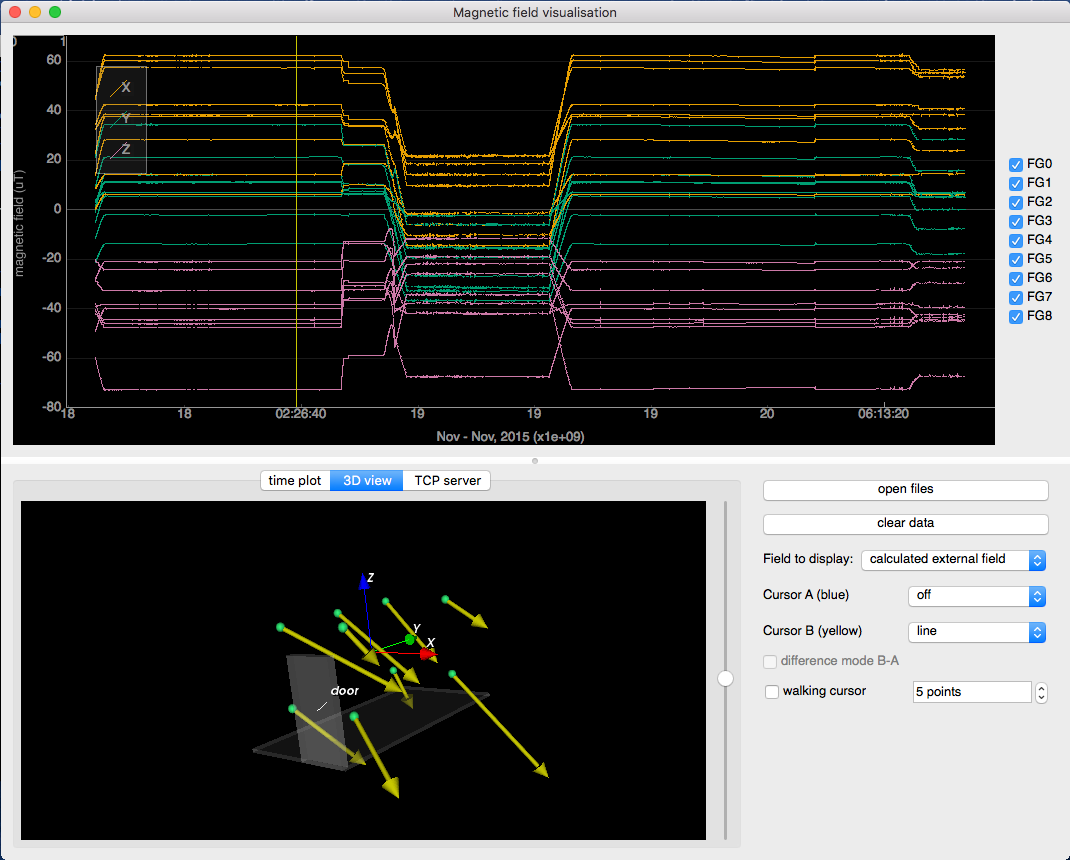
\includegraphics[width=0.8\linewidth]{gfx/nEDM_SFC/visualisation/visualisation1.png}
  \caption{Displaying the calculated back external field, the movable yellow cursor chooses the data to be displayed in the 3D view.}\label{fig:nEDM_SFC_visualisation1}
\end{figure}

Figure~\ref{fig:nEDM_SFC_visualisation1} shows the main window of the application. In the upper part the time series of the field is plotted, showing in the middle a sequence of ramps of the SULTAN magnet. The curves are grouped in colour by direction (x, y and z). In the figure the uncompensated field is plotted (Eq.\,\ref{eq:uncompensated_field}). One may also choose to plot the compensated, measured field. The plot features a vertical yellow cursor. It chooses the time for which a 3D visualisation of the field is displayed in the bottom area. Each sensor is depicted as a green sphere, from which an arrow points in the direction of the measured field, its length proportional to the field's magnitude. The view can be rotated.

% The overview can be seen in Fig.\,\ref{fig:nEDM_SFC_visualisation1}. There are two plot areas, upper in the time domain, lower can be switched between a 3D geometrical representation and a second time-domain plot. The loaded set of data, spanning 18-20 Nov 2015, shows a ramp of the SULTAN magnet. The ``field to display'' setting is set to ``calculated external field'', given by:
% \begin{equation}
%   \mathbb{B} - M \mathbb{I}
% \end{equation}
% Another option is displaying the measured field $\mathbb{B}$.
% In the first part the field points in the $x$ direction (North) and 45 degrees downwards (Villigen is 47 degrees in latitude). As expected for the Earth's magnetic field. On the upper plot there is a vertical yellow line, a movable cursor, that chooses which point in time is depicted in the 3D visualisation. There it visualises what is more-or-less the Earth's magnetic field at the experiment's position.

% \begin{figure}
%   \centering
%   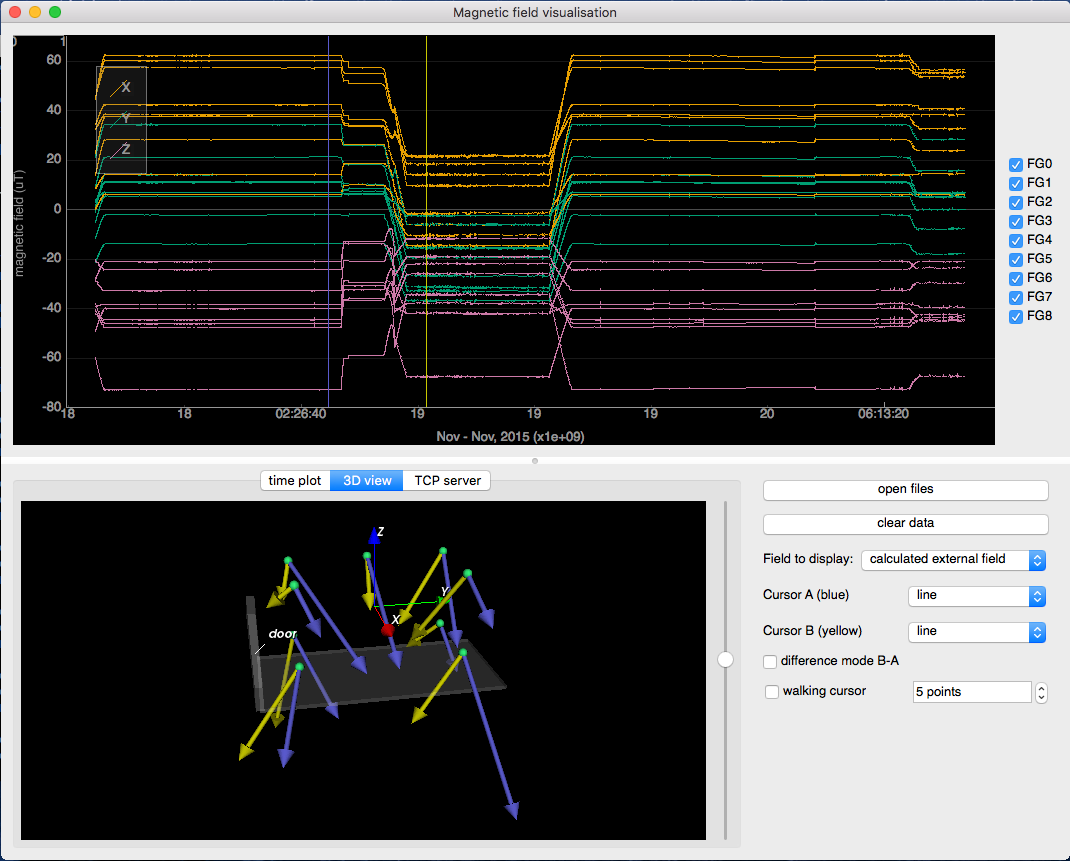
\includegraphics[width=0.8\linewidth]{gfx/nEDM_SFC/visualisation/visualisation2.png}
%   \caption{Displaying fields at two different times simultaneously, yellow and blue.}\label{fig:nEDM_SFC_visualisation2}
% \end{figure}

\begin{figure}
  \centering
  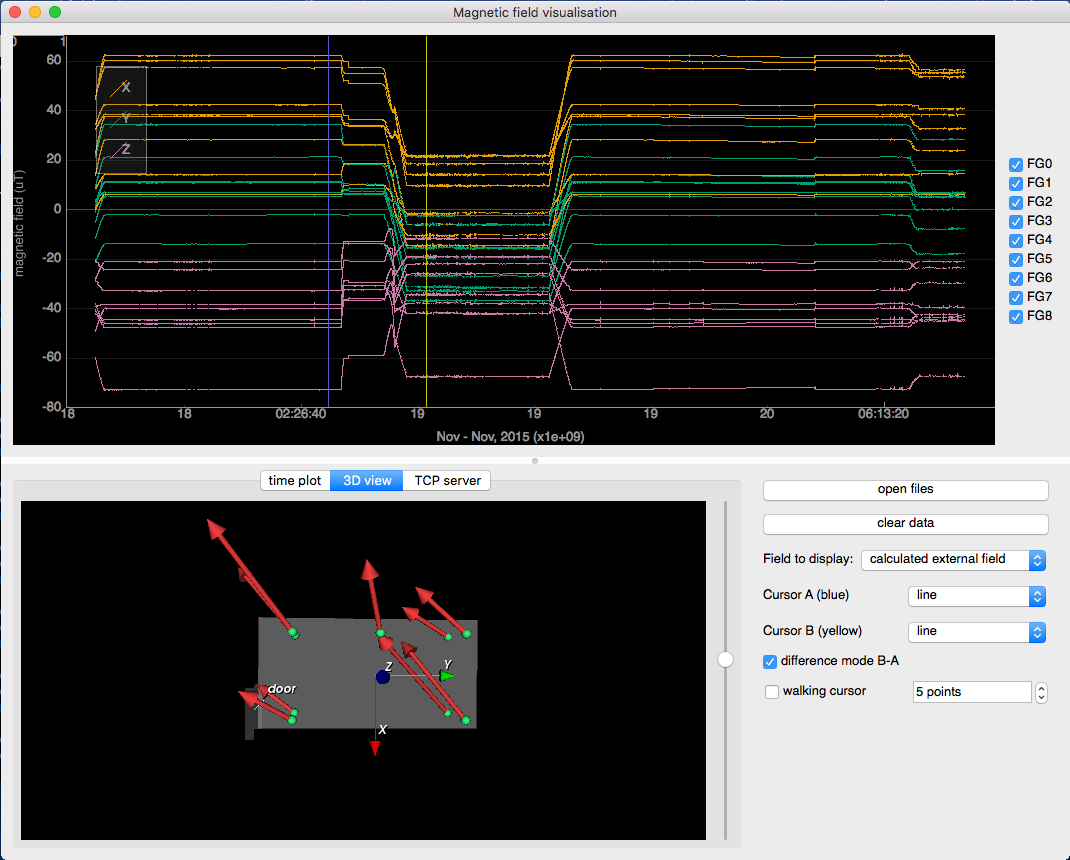
\includegraphics[width=0.8\linewidth]{gfx/nEDM_SFC/visualisation/visualisation4.png}
  \caption{Displaying the difference between the external field in two points in geometrical form.}\label{fig:nEDM_SFC_visualisation4}
\end{figure}

\begin{figure}
  \centering
  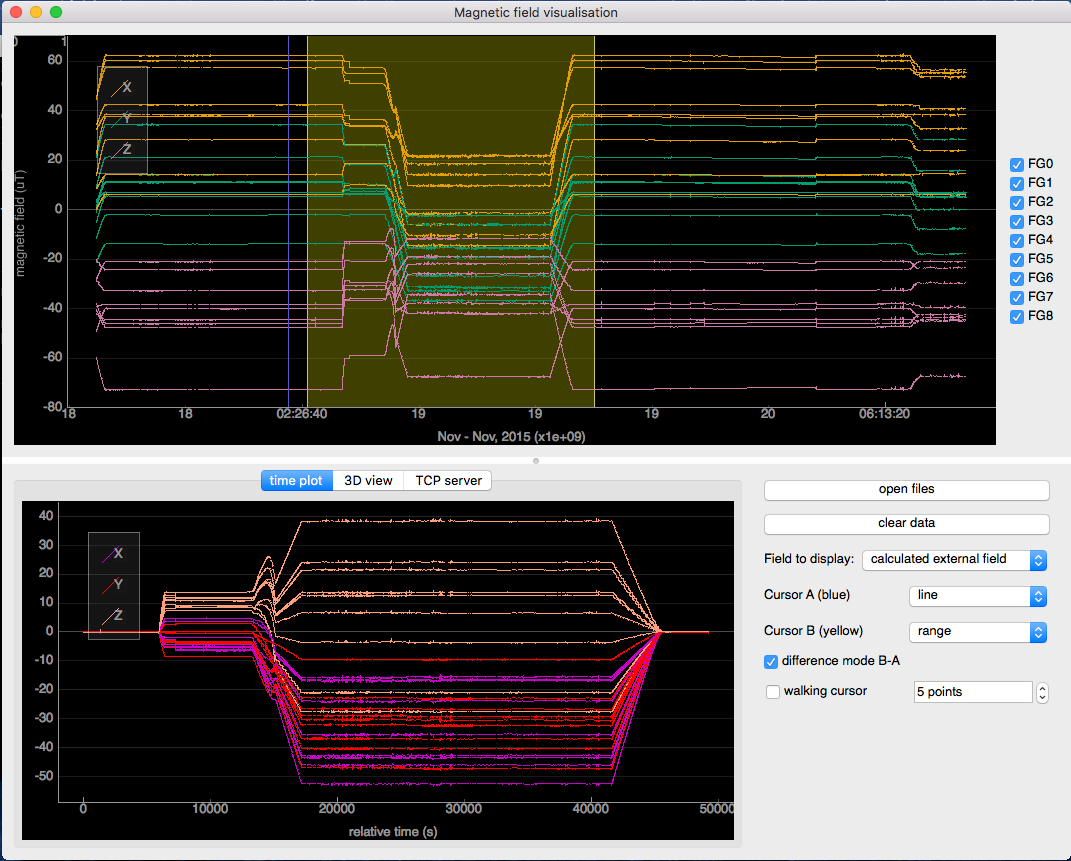
\includegraphics[width=0.8\linewidth]{gfx/nEDM_SFC/visualisation/visualisation3.png}
  \caption{Displaying a range of data, marked with the yellow cursor, relative to the point marked with the blue cursor. The calculated back external magnetic field is displayed.}\label{fig:nEDM_SFC_visualisation3}
\end{figure}

When two cursors are chosen, blue and yellow, the 3D view can also show the difference of the two. In Fig.\,\ref{fig:nEDM_SFC_visualisation4} the cursors are positioned before and after the ramp of the magnet, so that the difference corresponds to the field of the magnet only. In the 3D visualisation the direction in which the field points can be clearly seen.

Cursors can also mark a range of the data, the yellow one does in Fig.\,\ref{fig:nEDM_SFC_visualisation3}. The enlarged part is displayed relative to the field at the time chosen by the blue cursor in the upper area, in this case the field before the SULTAN ramp. So the bottom plot approximates the field of the SULTAN magnet, assuming there were no other changes of the field in that time. 

The application is cross-platform (Windows, OSX, Linux). It was written in python and uses the following libraries: Qt4 (cross-platform GUI), pyqtgraph (fast interactive plotting), VTK (3D graphics) and SciPy (data handling). It is a joint work with Nils Ebeling, for whom it was a summer project.






\chapter{Performance of SFC during SULTAN ramps}
Another task was to compare the SFC performance in shielding SULTAN ramps in 2015 and 2016. From a rather quick look at the data it seemed that the field inside the apparatus, as seen by the Hg comagnetometer and Cs magnetometers, was affected more strongly by the ramps in 2016 than in 2015.

% ((ext_field - B_Earth) * B_SULTAN)
The first is to determine the times of the ramps. Unfortunately, those data are not easily available. But could be calculated from the SFC data.

We define $\mathbb{B}_\text{Earth}$ as the uncompensated field ($\mathbb{B} - \mathbb{M} \mathbb{I}$) when the SULTAN magnet is known to be off. We then define the field of the SULTAN magnet to be $\mathbb{B}_\text{SULTAN} = \mathbb{B} - \mathbb{M} \mathbb{I} - \mathbb{B}_\text{Earth}$, when the magnet was known to be on. Then we can calculate the content of the SULTAN in the field by projecting the uncompensated field, minus the Earth's, on the one of the SULTAN\@:
\begin{equation}
  \left( \mathbb{B} - \mathbb{M} \mathbb{I} - \mathbb{B}_\text{Earth} \right) \cdot \mathbb{B}_\text{SULTAN}  
\end{equation}

\begin{figure}
  \centering
  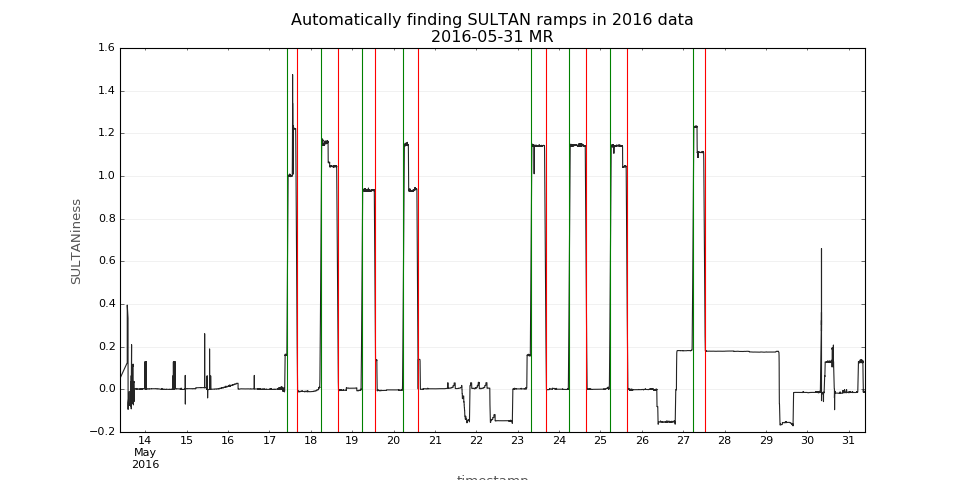
\includegraphics[width=.7\linewidth]{gfx/nEDM_SFC/finding_SULTAN_ramps.png}
  \caption
  [TODO]
  {\ldots}
  \label{fig:finding_SULTAN_ramps}
\end{figure}

The value of this projection for two weeks in May 2016 is depicted in Fig.\,\ref{fig:finding_SULTAN_ramps}. The SULTAN ramps are wonderfully pronounce and their times easy to get, as the times when the projection crosses 0.5 going up (ramp up) or down (ramp down).

\begin{figure}
  \centering
  \subfloat[Displaying the calculated back external field, the movable yellow cursor chooses the data to be displayed in the 3D view.]{
    \label{fig:SULTAN_ramp_Hg_performance}
    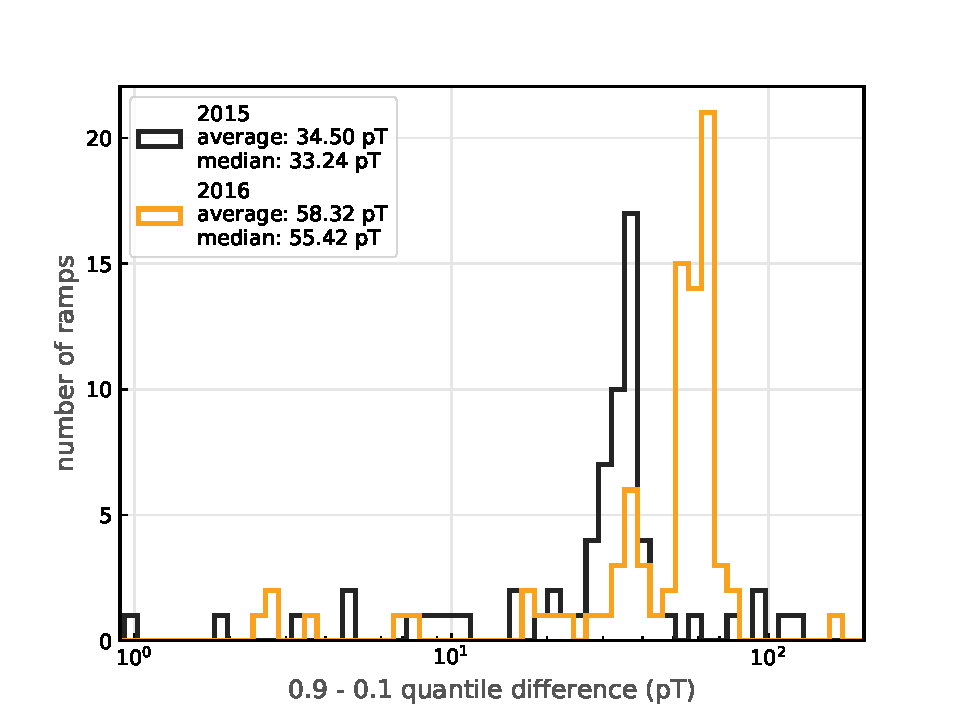
\includegraphics[width=.45\linewidth]{gfx/nEDM_SFC/field_seen_by_Hg_2015-2016}}
  \quad
  \subfloat[Displaying fields at two different times simultaneously, yellow and blue.]{
    \label{fig:SULTAN_ramp_Cs_performance}
    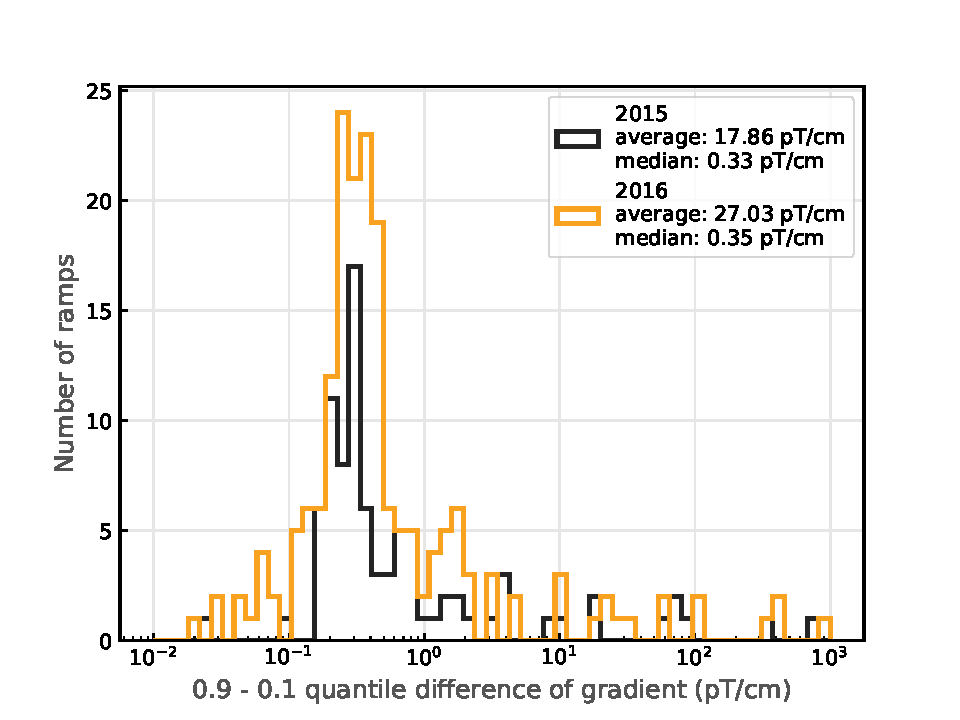
\includegraphics[width=.45\linewidth]{gfx/nEDM_SFC/gradient_seen_by_Cs_2015-2016}}
  \caption{Magnetic field of the SC magnet seen by the SFC. Taken as difference of runs... \note{make the plots nicer, no vertical scale, no grid, filled histograms.}}
\end{figure}

With the exact times of the SULTAN ramps available, the Hg comagnetometer and Cs magnetometer data in a 2h window around each of the ramps were taken. From the Cs data the gradient was estimated as the difference between the averages of the top and bottom sensors, divided by the separation of \SI{25.1}{\centi\meter}. The change was defined as 0.9 and 0.1 quantile difference. The histogram for all the field changes, as measured by the Hg, during SULTAN ramps is shown in Fig.\,\ref{fig:SULTAN_ramp_Hg_performance}. It is visible that while in 2015 the changes are consistently around \SI{34}{\pico\tesla}, in 2016 the changes are centred around \SI{55}{\pico\tesla}.

\note{Look once again into the data, try to see what the peak is.}

\note{Write that the scheme may be more generally used?}

Conclusion: reason is unknown, but the incentive to find it out is not to strong. Changes in the field are compensated by the Hg magnetometer. The uncompensated vertical gradient change remained the same.






% \section{Influence of the SC magnet}
% The ultracold neutrons are polarised by passing through a superconducting magnet. The length of the path of the neutrons to the experiment should be small to minimise transport losses. For this reason the experiment is located close to the exit of the UCN beam--port and the magnet is fit in between.

% \begin{figure}
%   \centering
%   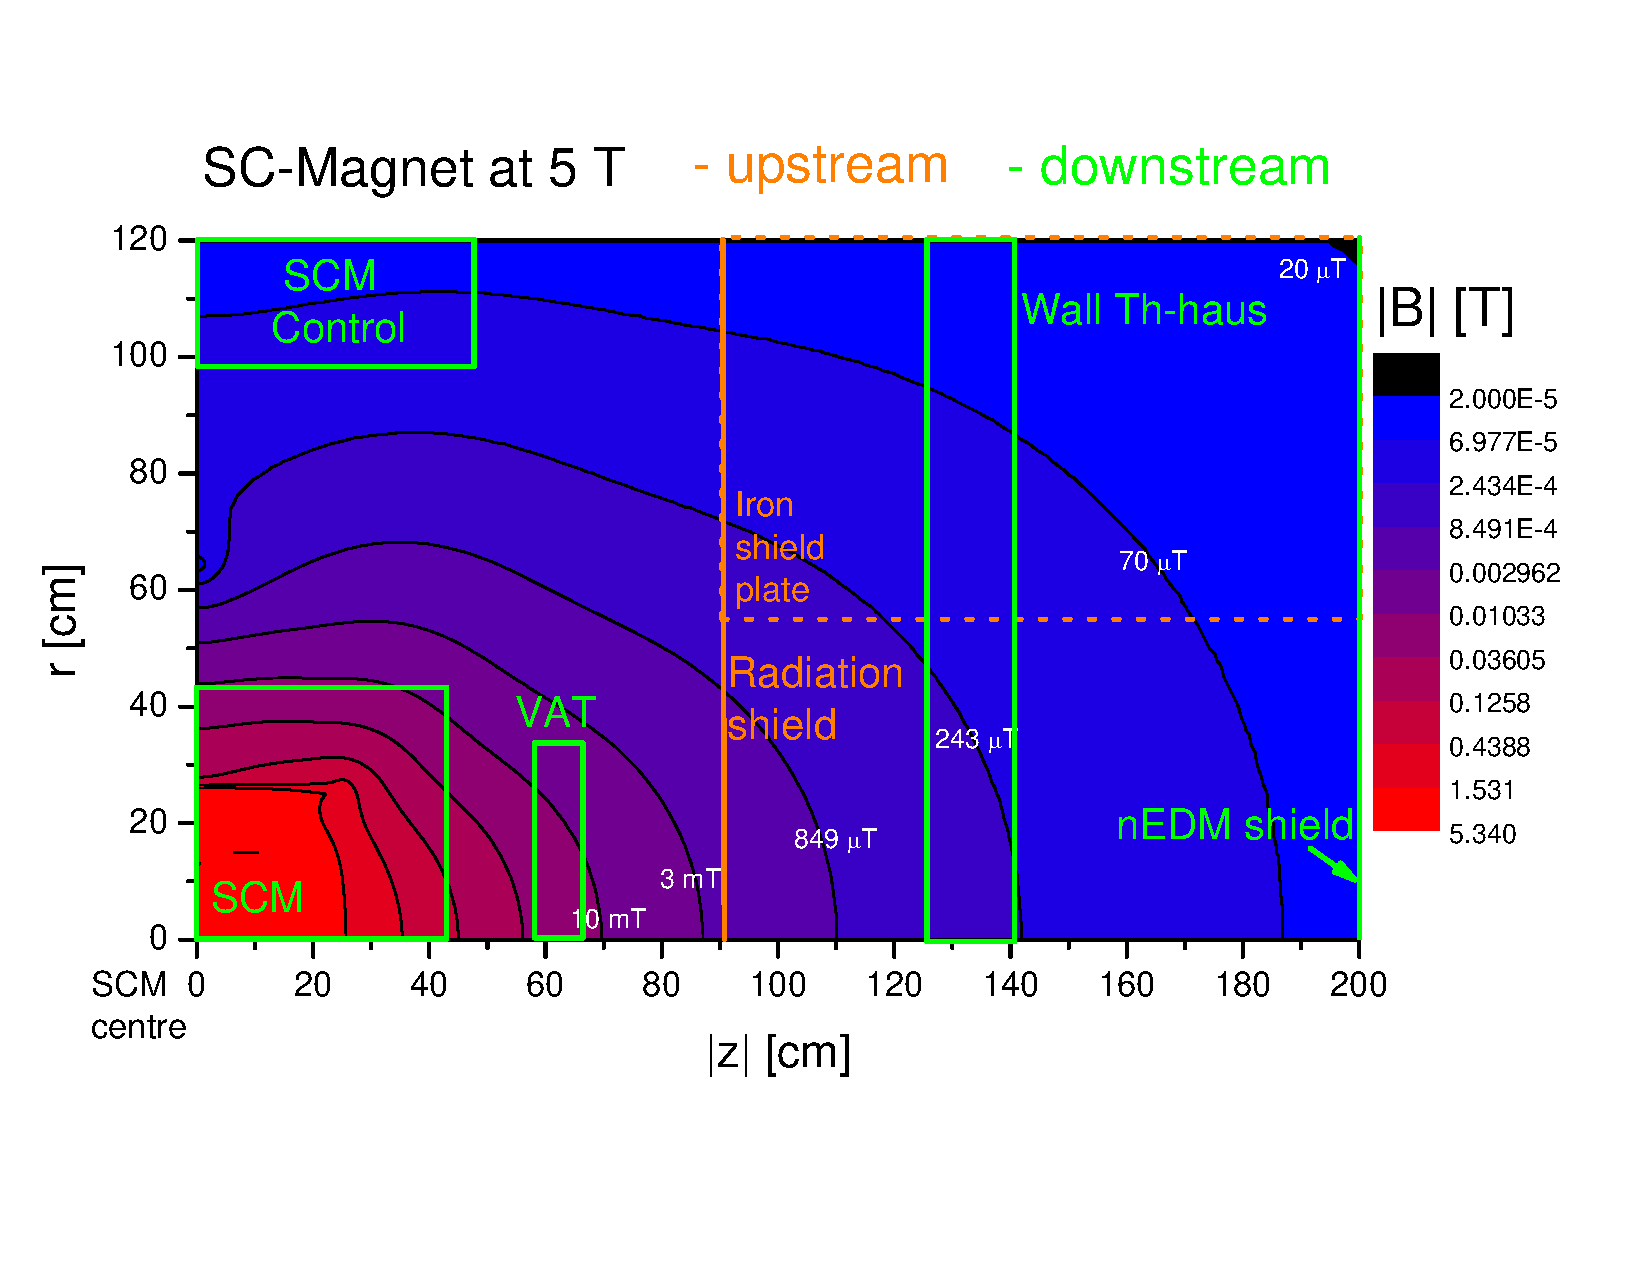
\includegraphics[width=.7\linewidth]{gfx/nEDM_SFC/SCM_magn_map.pdf}
%   \caption
%   [TODO]
%   {Map of the magnetic field of the superconducting magnet. Courtesy of Dr. Geza Zsigmond}
%   \label{fig:nEDM_SFC_SC_magnet_map}
% \end{figure}

% \begin{figure}
%   \centering
%   \subfloat[Displaying the calculated back external field, the movable yellow cursor chooses the data to be displayed in the 3D view.]{
%     \label{fig:nEDM_SFC_SC_magnet_influence_top_view}
%     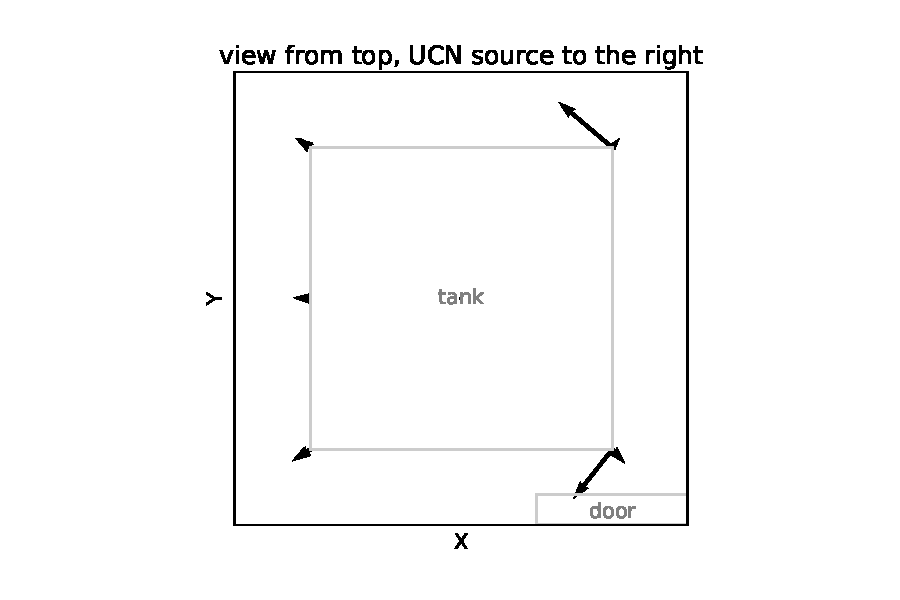
\includegraphics[width=.45\linewidth]{gfx/nEDM_SFC/SC_magnet_field_top_view.pdf}}
%   \quad
%   \subfloat[Displaying fields at two different times simultaneously, yellow and blue.]{
%     \label{fig:nEDM_SFC_SC_magnet_influence_front_view}
%     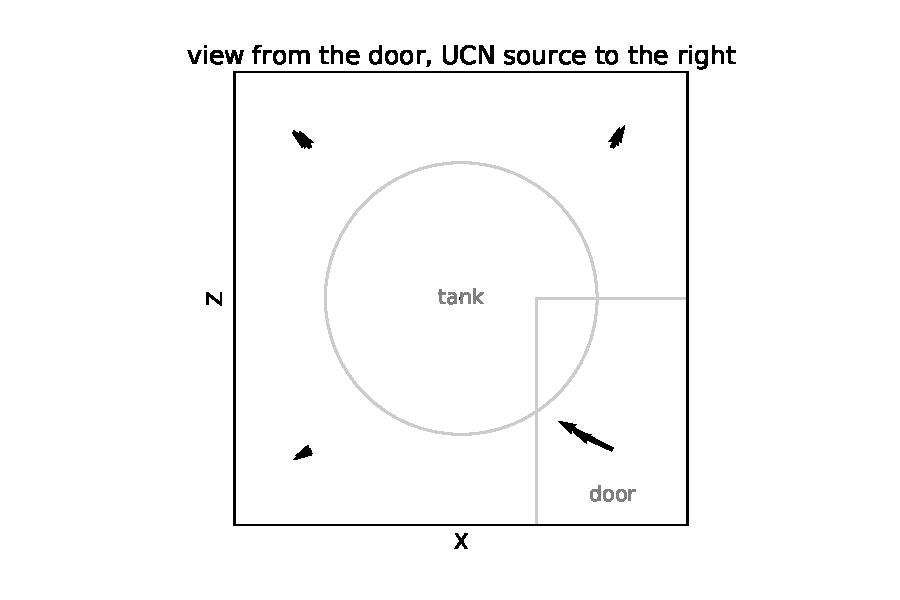
\includegraphics[width=.45\linewidth]{gfx/nEDM_SFC/SC_magnet_field_front_view.pdf}}
%   \caption{Magnetic field of the SC magnet seen by the SFC. Taken as difference of runs...}
% \end{figure}

% \begin{figure}
%   \centering
%   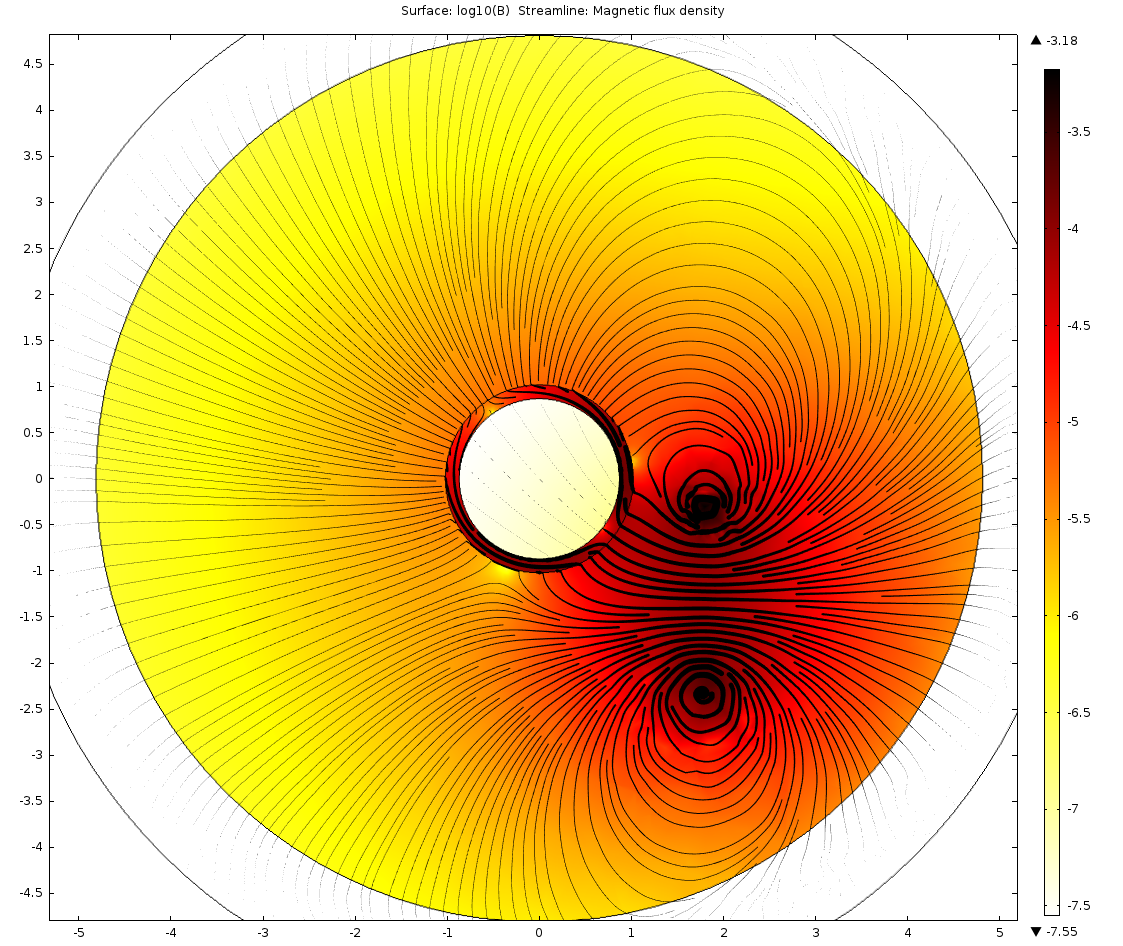
\includegraphics[width=.7\linewidth]{gfx/nEDM_SFC/SC_magnet_optimal_coil_on_wall.png}
%   \caption
%   [TODO]
%   {Map of the field of a potential correcting coil}
%   \label{fig:nEDM_SFC_SC_magnet_optimal_coil}
% \end{figure}

% \begin{figure}
%   \centering
%   \subfloat[Displaying the calculated back external field, the movable yellow cursor chooses the data to be displayed in the 3D view.]{
%     \label{fig:nEDM_SFC_SC_magnet_influence_top_view2}
%     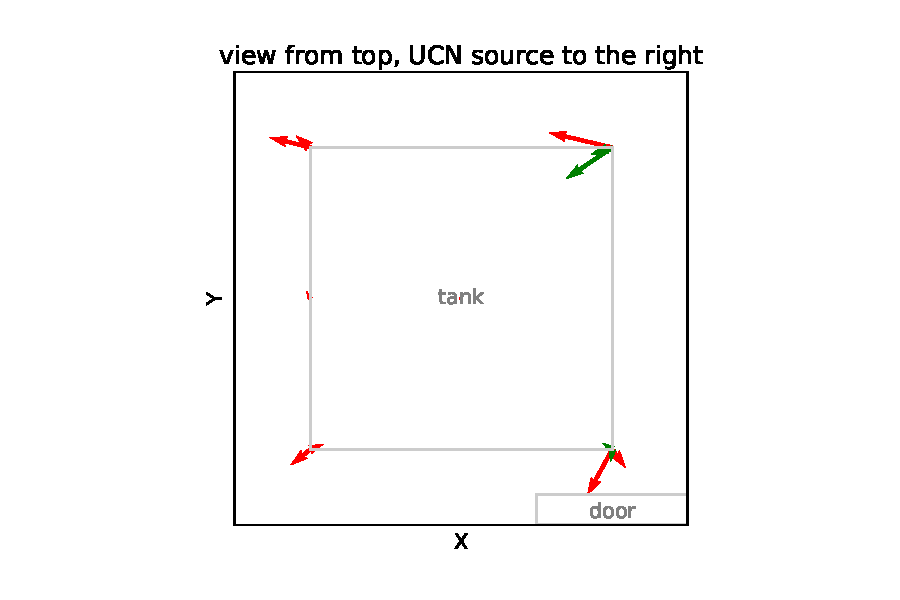
\includegraphics[width=.45\linewidth]{gfx/nEDM_SFC/SC_magnet_improvement_top_view.pdf}}
%   \quad
%   \subfloat[Displaying fields at two different times simultaneously, yellow and blue.]{
%     \label{fig:nEDM_SFC_SC_magnet_influence_front_view2}
%     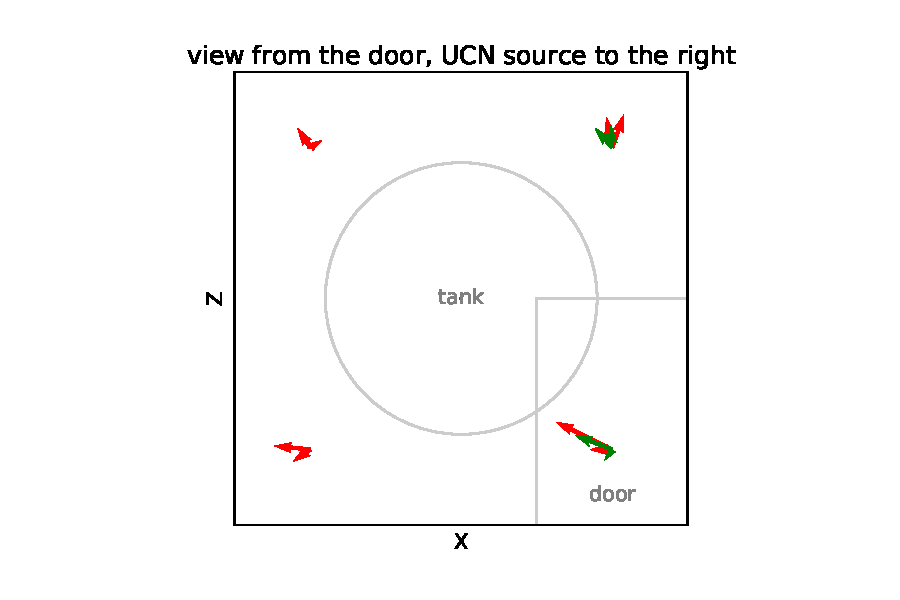
\includegraphics[width=.45\linewidth]{gfx/nEDM_SFC/SC_magnet_improvement_front_view.pdf}}
%   \caption{Magnetic field of the SC magnet seen by the SFC. Taken as difference of runs...}
% \end{figure}

% The improvement in the range of the field is 40-70\% (In different simulated runs, 21.7 to 12.6 (42\%), 22.2 to 12.9 (42\%), 19.3 to 5.8 (70\%), and 35.1 to 18.6 (57\%)), unit microteslas.


\chapter{Magnetic field during sparks in the high-voltage system}

\note{Push it into an appendix?}

This is important! As clearly the most dangerous magnetic fields are ones correlated with HV.

The resistor to limit the current. It is a spiral of chained small resistors, submerged in cooling oil.

\begin{figure}
  \centering
  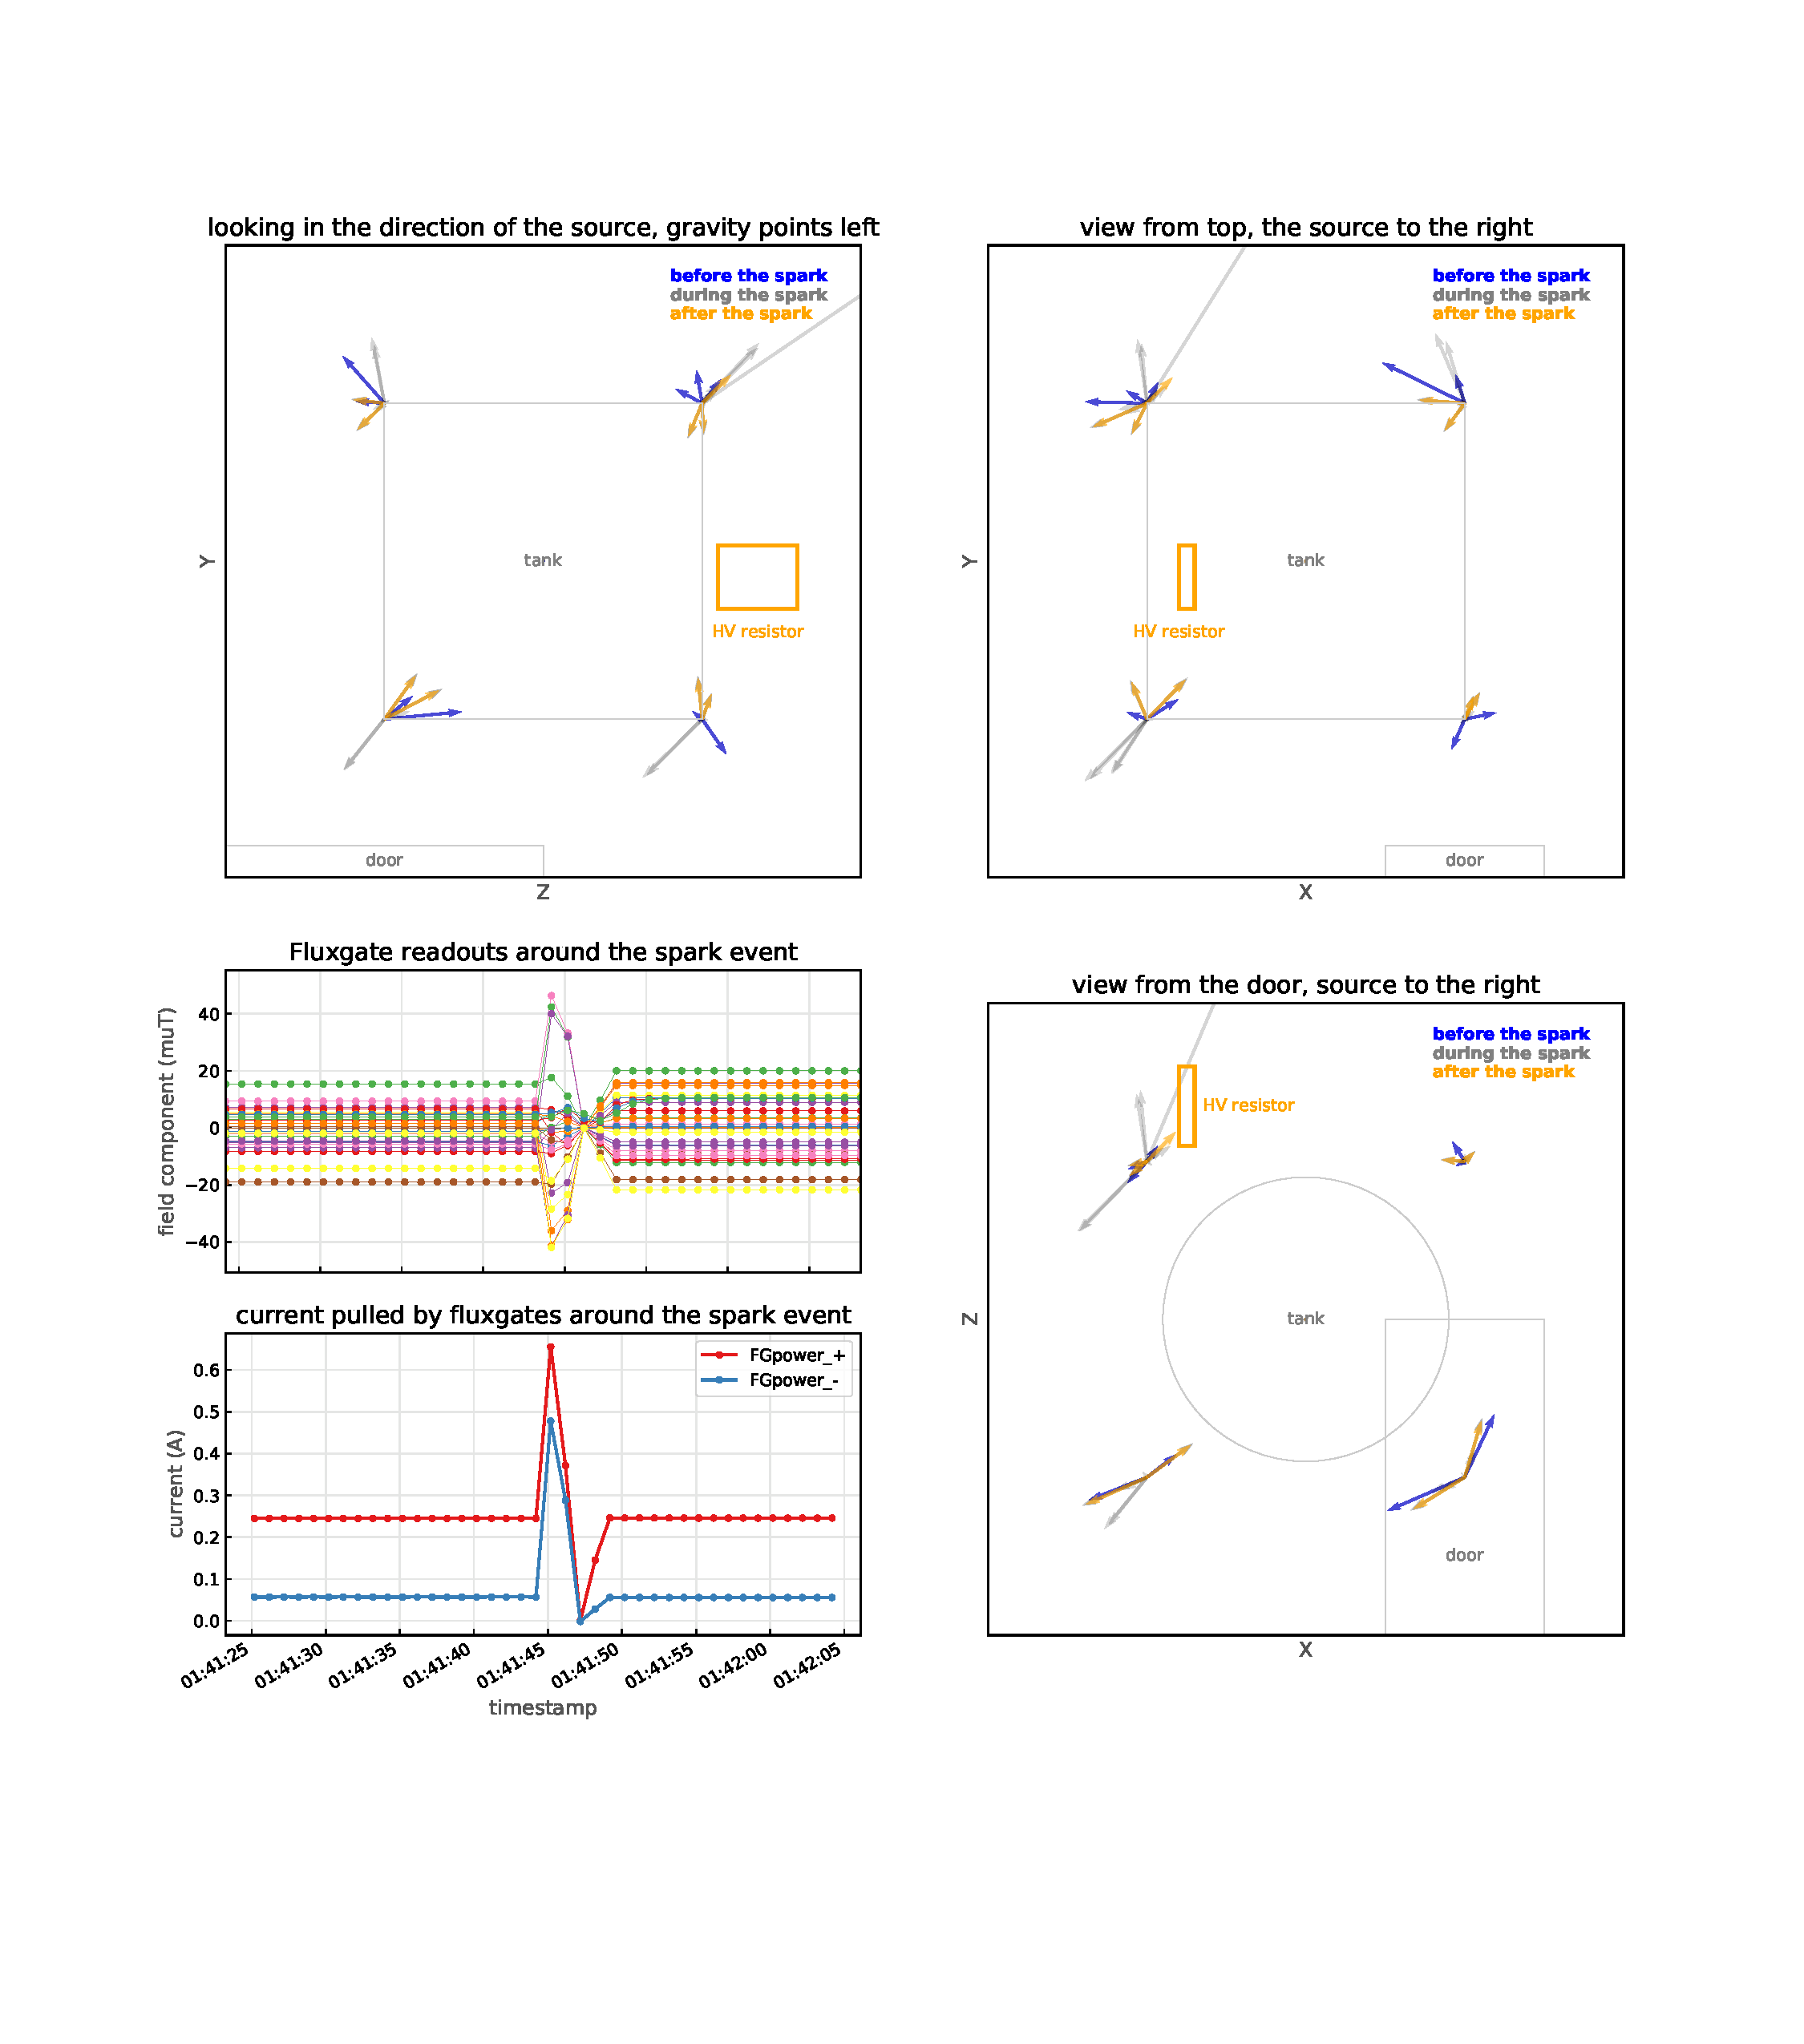
\includegraphics[width=\linewidth]{gfx/nEDM_SFC/SFC_during_spark_event_thesis.pdf}
  \caption
  [TODO]
  {\ldots}
  \label{fig:field_when_sparking}
\end{figure}


Fortunately, HV was very stable during the data taking and sparks hardly ever happend.

\note{How can I learn how often we had sparks?}









% \section{Optimising the number of windings in the coils}
% Put the plots of the distributions of the currents, juxtapose them with the
% ranges of the power supplies.